\section{Model Stability} \label{stability}

\subsection{Integration in SPICE}

SPICE implementations in general rely on second-order integration, namely trapezoidal and Gear integration. LTspice allows the user to pick between 4 options: trapezoidal,
Gear, (1st Order) Backward Euler and a proprietary modified trapezoidal method. In general,
Backwards is the most stable and least accurate, followed by Gear integration 
\cite{ltspice-diff-post, spice-book}.

Trapezoidal integration is generally faster and more accurate than gear but introduces a ringing
numerical artifact that occurs at adjacent timesteps on stiff systems. Ringing is dampened by the gear
method causing this numerical artifact to be mostly eliminated. The gear method achieves that by
dampening most ringing as shown in figure \ref{fig:trapz_vs_gear}. The setup in figure \ref{fig:trapz_vs_gear} uses an nanowire-capacitor oscillator working in the linear regime starting
with an initial amount of energy.
We typically care about oscillatory behavior in nanowires that can be filtered by the gear
method (especially in the timeframe shown)
and as a result, we choose to use the trapezoidal method. LTspice's 
default integration method is a proprietary modified version of trapezoidal integration 
that cancels out the trapezoidal ringing introduced by the regular implementation without
numerical dampening \cite{ltspice-diff-post}. 

\begin{figure}
    \centering
    \subfigure[]{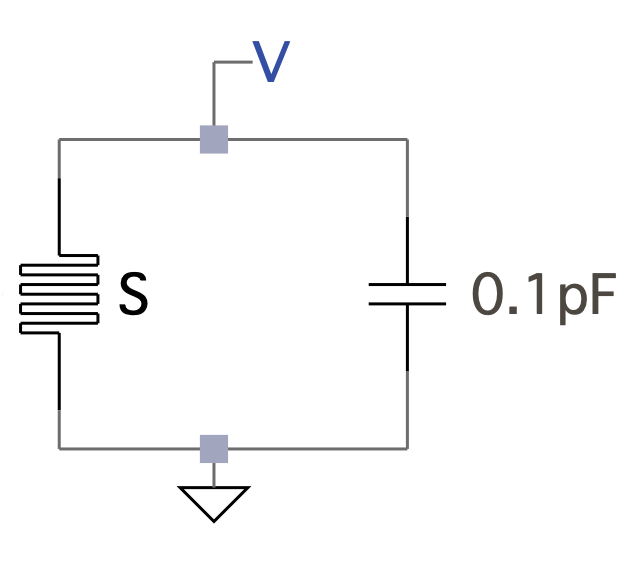
\includegraphics[width=0.3\textwidth]{figs/method_vs_Circ.png} \label{fig:tank_circ}}
    \subfigure[]{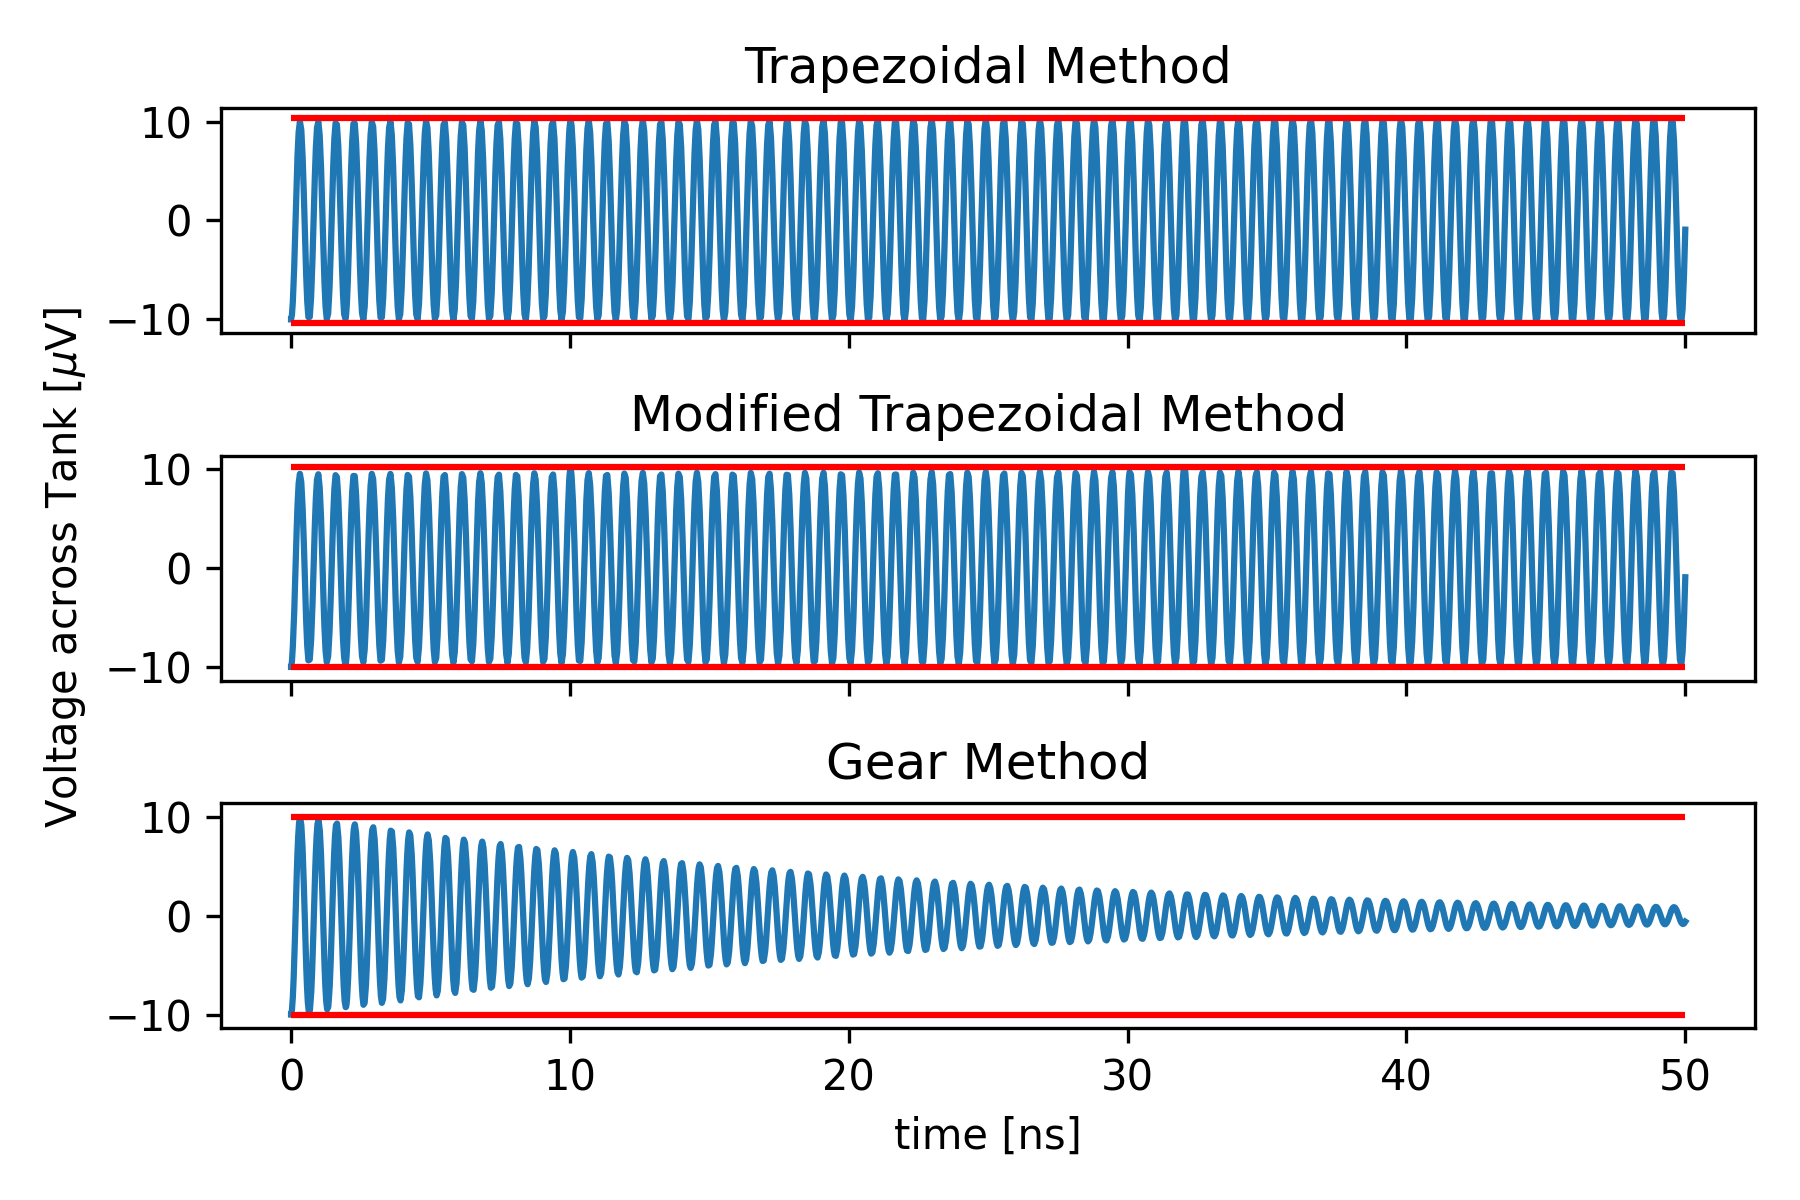
\includegraphics[width=0.67\textwidth]{figs/method_vs.png}}
    \caption{Comparison of the 3 different second-order integration methods
    LTspice is equipped to use. (a) An LC resonator that uses a non-linear inductor
    (nanowire) in parallel with a capacitor. The initial condition for node \cf{V} is set
    to $100\mu$V.
    (b) The voltage as a function of time
    computed using the 3 different integration methods. Gear method causes significant
    signal decay when there shouldn't be decay at timescales we typically care about 
    in nanowires. The modified trapezoidal method
    has less consistent magnitudes of the output sine wave.}
    \label{fig:trapz_vs_gear}
\end{figure}

\subsection{Stability in Transient Simulations}

Stability of a finite element method is intimately related to the consistency and convergence of
the method through the Dahlquist Equivalence Theorem \cite{DAHLQUIST}. 
One result of this for non-linear systems,
such as the nanowire model, is their solution should be smooth as you decrease the timestep.
As in, there must exist a timestep $\Delta t$ for which all timesteps $< \Delta t$ the method
gives a result bounded around that of using the timestep $\Delta t$. Transient simulations, which are a 
type of continuation method parametrized with time, often use straightforward convergence correction. 
In this method, the timestep for continuous signals is decreased until convergence is achieved, 
which is guaranteed to occur for continuous signals \cite{spice-book}.

One way of visualizing solving a continuous system using a finite element method is by
represent timestep corrections
as projections. For instance, solving for the final state $u(T)$ for a circuit $C$ at a time $T$ 
transforms $u(0)\xrightarrow[]{} u(T)$ smoothly when continuous. However, when a finite method is used
with coarse discretizations, the method steps around this continuous evolution. Overshoots due to the
coarseness could exist outside the state-space and the solution trajectory but are corrected for
as illustrated in figure \ref{fig:statespaceevolution}. 
These corrections (decreasing the timestep and adding gmin capacitances) can be thought of as projections
back into the subspace of possible solutions. The subspace of possible solutions is
a lightcone around the current state where the size of the lightcone is constrained
by the circuit topology and simulation parameters such as \cf{reltol}. The lightcone
of a state is the set of states you can reach from that state in one timstep. The
lightcone of a target state is the set of states that can reach it in one timestep.

In a non-linear system, these projections can lead to integrating errors. Consider the
state non-linearity for instance, if a projection happens to enter that regime at any
point in the simulation accidentally, it would cause a misfire. Now consider the coupling
of this to the continuous non-linearity which amplifies values. This amplification can
make it easier to reach the state non-linearity lightcone and accidentally trigger
the hotspot integrator.

\begin{figure}
    \centering
    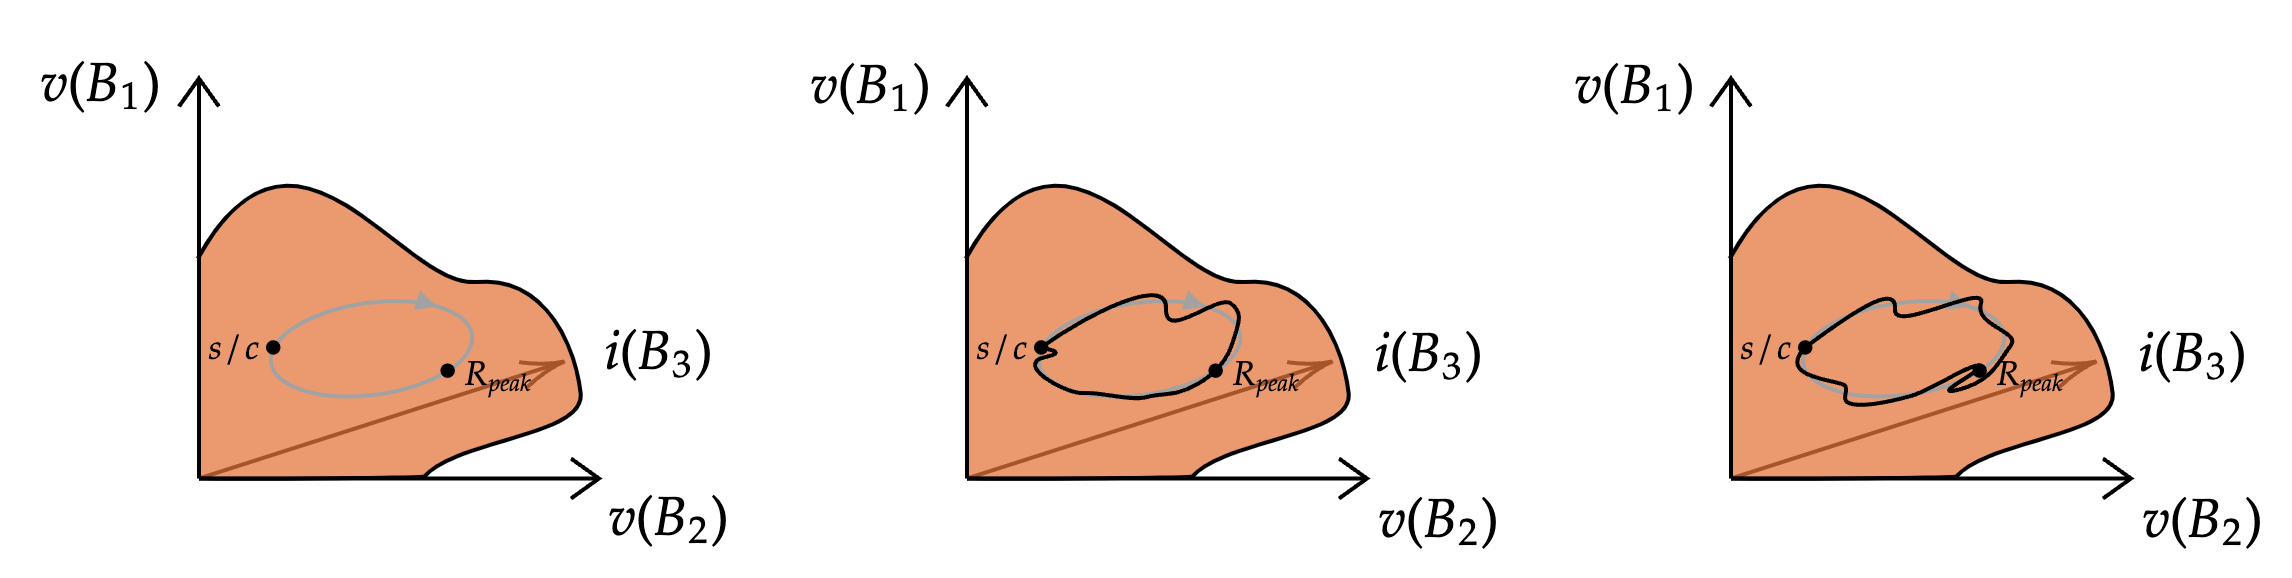
\includegraphics[width=0.9\textwidth]{figs/statespaceevolution.png}
    \caption{A diagram of the evolution of a circuit simulation for a nanowire.
    The orange space represents all the states (combinations of node voltages and currents) 
    that the circuit can be in. [TODO FINISH THIS conceptual/notional diagram]}
    \label{fig:statespaceevolution}
\end{figure}

\subsubsection{Stability of the Nanowire Model} 

Boolean state non-linearities are integral to optimizing and training Neural Networks, and as a 
result are a well studied concept. A common way of solving this issue is smoothening out the 
change by modeling the boolean state as a continuous state transition with a smooth interpolating
function, such as a sigmoid function. In nanowires, we particularly care about smoothness of state
transition over time while the transition dependence is on current (which is also a function of time).
Macroscopically, this state transition involves a chain reaction and can be modelled as a smooth
ramp up (the hotspot thermal growth is a smooth change). This is how the hotspot integrator in the 
existing nanowire model handles the non-linear transition into the resistive state.

The nanowire model is unstable and inconsistent over both types of non-linearities in a disguised 
fashion. While this can be improved by tweaking the relative tolerance (\cf{reltol}) 
of the simulation, improving the model's stability is essential to scaling devices and integration 
with other circuits.
One big issue with the instability is the behavior of the model is not out of question, in that,
even though the solution is incorrect, it looks plausible. For instance, you might see extra counts
when you aren't supposed to see them when you include tapers (due to the modified time-stepping behavior
for circuits when tapers are included, discussed in \ref{tapers_section}). Other instability effects
include things like pre- and post-firing of the nanowire, which can be hard to discern from reflections
occurring in the circuit that might actually cause the wire to re-fire.

This instability over the non-linearity is amplified due to the time-stepping. An approximate 
solution to a non-linear system has a response dependent on the magnitude at the previous timestep. 
As a result,
near portions of the transfer functions that can't be approximated as linear, a projection
onto an acceptible relative tolerance value at timestep $n$ does not correspond to an
acceptable relative tolerance at a timestep $n+1$ due to the magnitude dependence.
This forward propagation of error explains false switching events at timesteps that
are too close together caused by a time-coupled element (more on that in \ref{malicious_circuits}.
We see this in effect in figure \ref{fig:sweepbias} with multiple false switching events.

\subsubsection{Relative Tolerance for the Nanowire Model} \label{reltol}

\begin{figure}
    \centering
    % \subfigure[]{
    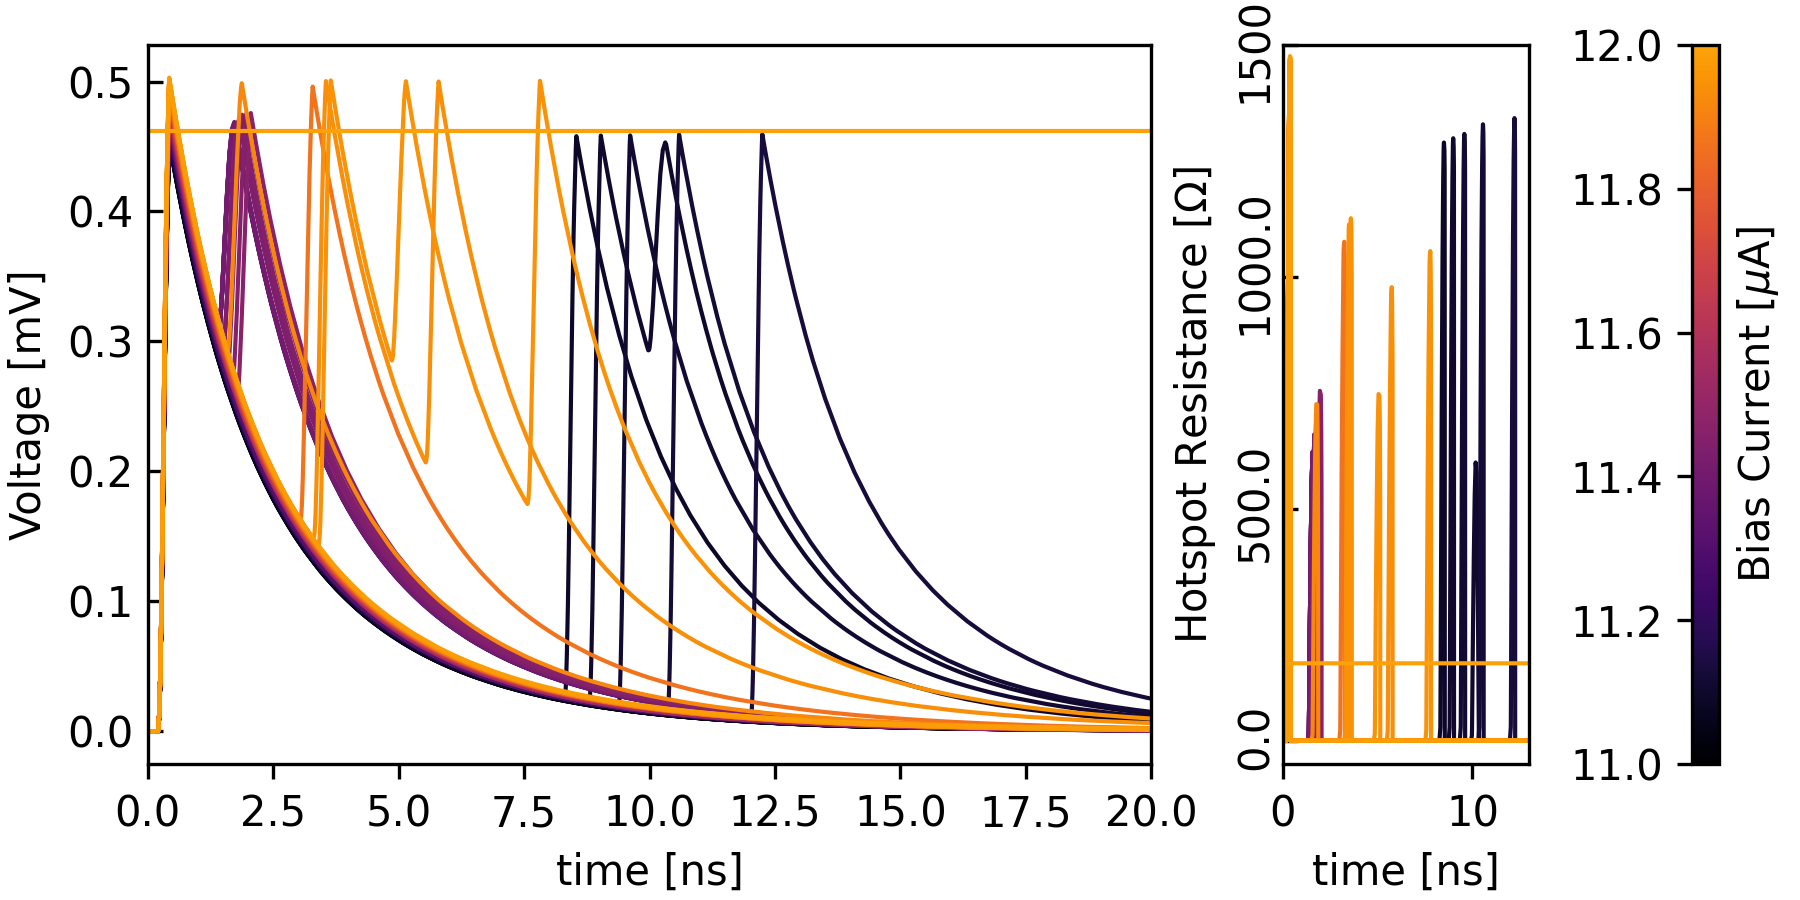
\includegraphics[width=0.8\textwidth]{figs/jumbled_mess_new.png}
    % }
    \caption{SNSPD readout circuit tested against 100 different bias values between
    $11\mu$A and $12\mu$A for a device with switching current $12\mu$A. The simulation
    was carried out using the existing nanowire model and the default options for LTspice
    on Mac (\cf{reltol} of $10^{-3}$, \cf{voltol} of $10^{-6}$, \cf{trtol} of $2$). 
    We expect to see only
    one pulse at $10$ns for all biases (except $12\mu$A). The instability of the model is
    related to the ratio of correct and incorrect simulations.}
    \label{fig:sweepbias}
\end{figure}

% these references are not as good, but may be worth checking out?
% https://gist.github.com/turingbirds/c90672c3b126d0d5f37f90494d5057cb
% https://www.eevblog.com/forum/projects/lt-spice-convergence/

Relative tolerance in SPICE is a simulation parameter that imposes a convergence criterion.
It is typically imposed in the form \cite{accurate_sim_in_spice_kundert}:
$$|v_{k+1} - v_k| \leq \cf{reltol} \cdot \max(|v_{k+1}|, |v_k|) + \cf{vntol}$$

This imposes a condition on the node voltage $v_i$ change between iterations $k$ and $k+1$.
\cf{vntol} is equivalent to the voltage resolution and should be at least one order of magnitude
smaller than any node voltage (including the thermal integrator, more on that in section
\ref{current_nw}. Even though the nanowire might be a 2-port element (ignoring the photon port),
the relative tolerance is check on the entire subcircuit. This implies that the relative
tolerance needs to satisfy this constraint on all logic inside the nanowire.

\subsubsection{Behavioral Sources}

Dependent sources are a powerful model in SPICE software that allows their output to be
dependent on other node voltages and currents. Along with the multiple types
of dependent sources that are supported by SPICE (e-, f-, g- and h-sources), LTspice
supports an additional type of dependent source called the behavioral source (b-source).
Behavioral sources can mimic the behavior of any other source type and additionally
can have multiple inputs (as opposed to the other sources' dependence on only one value).
B-sources also allow for the use of arbitrary maths functions that allow them to compute
non-trivial expressions, such as time integrals, derivatives and modulos.
B-sources can use the outputs of functions defined using the \cf{.func} directive
as a current, voltage, resistance and power outputs (resistance and power aren't well 
documented). 

\begin{figure}
    \centering
    \subfigure[]{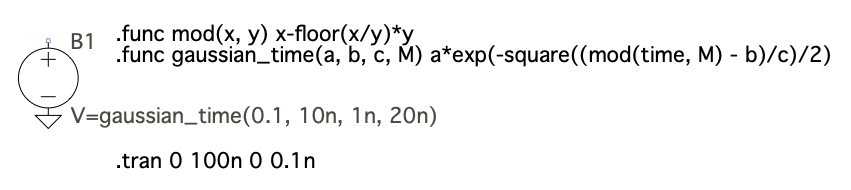
\includegraphics[width=0.8\textwidth]{figs/gaussian_src_circuit.png}
    \label{fig:gaussian_src_circ}}
    \subfigure[]{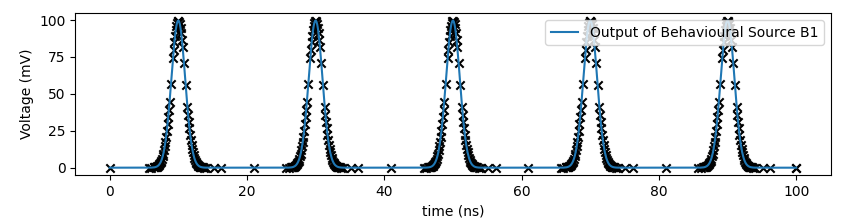
\includegraphics[width=0.8\textwidth]{figs/gaussian_src_output.png}
    \label{fig:gaussian_src_out}}
    \caption{Example of a behavioral source outputting gaussian pulses.}
\end{figure}

For example, one can construct a gaussian pulse source using dependent sources
by defining the two functions \cf{mod} and \cf{gaussian\_time} as shown in 
\ref{fig:gaussian_src_circ}.
% \begin{lstlisting}[language=python]
% .func mod(x, y) x-floor(x/y)*y
% .func gaussian_time(a, b, c, M) a*exp(-square((mod(time, M)-b)/c)/2)
% \end{lstlisting}
Using a b-source expression \cf{V=gaussian\_time(0.1, 10n, 1n, 20n)}
outputs a gaussian pulse with magnitude $0.1V$ with peaks
spaced out by $10$ns with a standard deviation of $1$ns as shown in figure
\ref{fig:gaussian_src_out}. 

B-sources are a helpful tool when designing circuits for stability as they
allow you to abstract complexity away from the circuit topology and remove 
reliance on \cf{reltol}. They can also function as state variables and perform
maths on expressions that have varying output values -- such as performing maths
on outputs that differ by more than 6 orders of magnitude. 

\subsection{Malicious Circuits} \label{malicious_circuits}

One method proposed to test for the stability of a nanowire model is by enumerating
the number of false switching events. In the same fashion that the state nonlinearity
can be used to amplify single events of small magnitude, the model can be used to 
nanowire count erroneous state crossings. If a simulation $\Sigma_C$
of a nanowire circuit $C$ accesses a state $\Sigma_C( u(t=0), T ) = u(T)$ after
a time $T$ using a finite method,
then running the same method with more steps should yield $u(T)$ if the method
converges \cite{DAHLQUIST}.
However, if the projections taken between simulation steps due to criterion 
based convergence introduce some deviation $\varepsilon$ at time $t'$ from the 
true circuit state, then the final solution will evolve from an $\varepsilon$ lightcone
away from $u_C(t')$. In a linear system, the $\varepsilon$ lightcone might be hard to
distinguish as $\Sigma_C(u(t=0), T) + \Sigma_C(\varepsilon, T-t') \approx \Sigma_C(u(t=0), T)$. 

However, since the nanowire's state is non-linear, if the $\varepsilon$ deviation happens
near a switching event, then the projection has a probability of switching the 
nanowire. By enumerating simulations of a nanowire varying the timestepping,
we can force the find the frequency of $\varepsilon$ errors occuring from switching
events.

Unfortunately, we can't perform this enumeration by varying timesteps in LTspice 
trivially. One workaround however, is simulating a circuit $C'=C+M$ that contains
the original circuit $C$ and a new malicious circuit $M$. $M$ doesn't have to be coupled
to $C$ topologically ($M$ and $C$ share no nodes, currents or behavioural coupling).
However, $C$ and $M$ are now time coupled, in that if $M$ exhibits a strong non-linearity
then the simulation of $C$ also experiences finer timesteps. This time coupling allows
for enumerating simulations of $C$ without manually modifying the timesteps taken.

One example malicious circuit $M$ could be a voltage source exhibiting a pulse 
with a magnitude at least as big as $(\cf{voltol})/(\cf{reltol})$\todo[]{verify this ratio}
as shown in figure \ref{fig:w_malicious_circ_diag}.
This forces the simulator to use finer steps near the ppulse edges and as a result
introduces some timestep variation to $C$ as well. Another example malicious circuit 
could be a one-way coupled circuit, such as a behavioural source whos output is coupled
to a node in $C$ and amplifies its magnitude. This is equivalent to having the simulation
tolerances be different for one node in the circuit.

A special case for $M$ is the transmission line. The inclusion of a transmission line
in SPICE creates breakpoints that force the timestepping resolution for the entire simulation
to be below half the total line delay \cite{hspice, spice-book}. One possible enumeration would
be varying the delay of an \cf{LTRA} (O- or T-models). This works even when the transmission line
is not connected to anything.

\begin{figure}
    \centering
    \subfigure[]{
    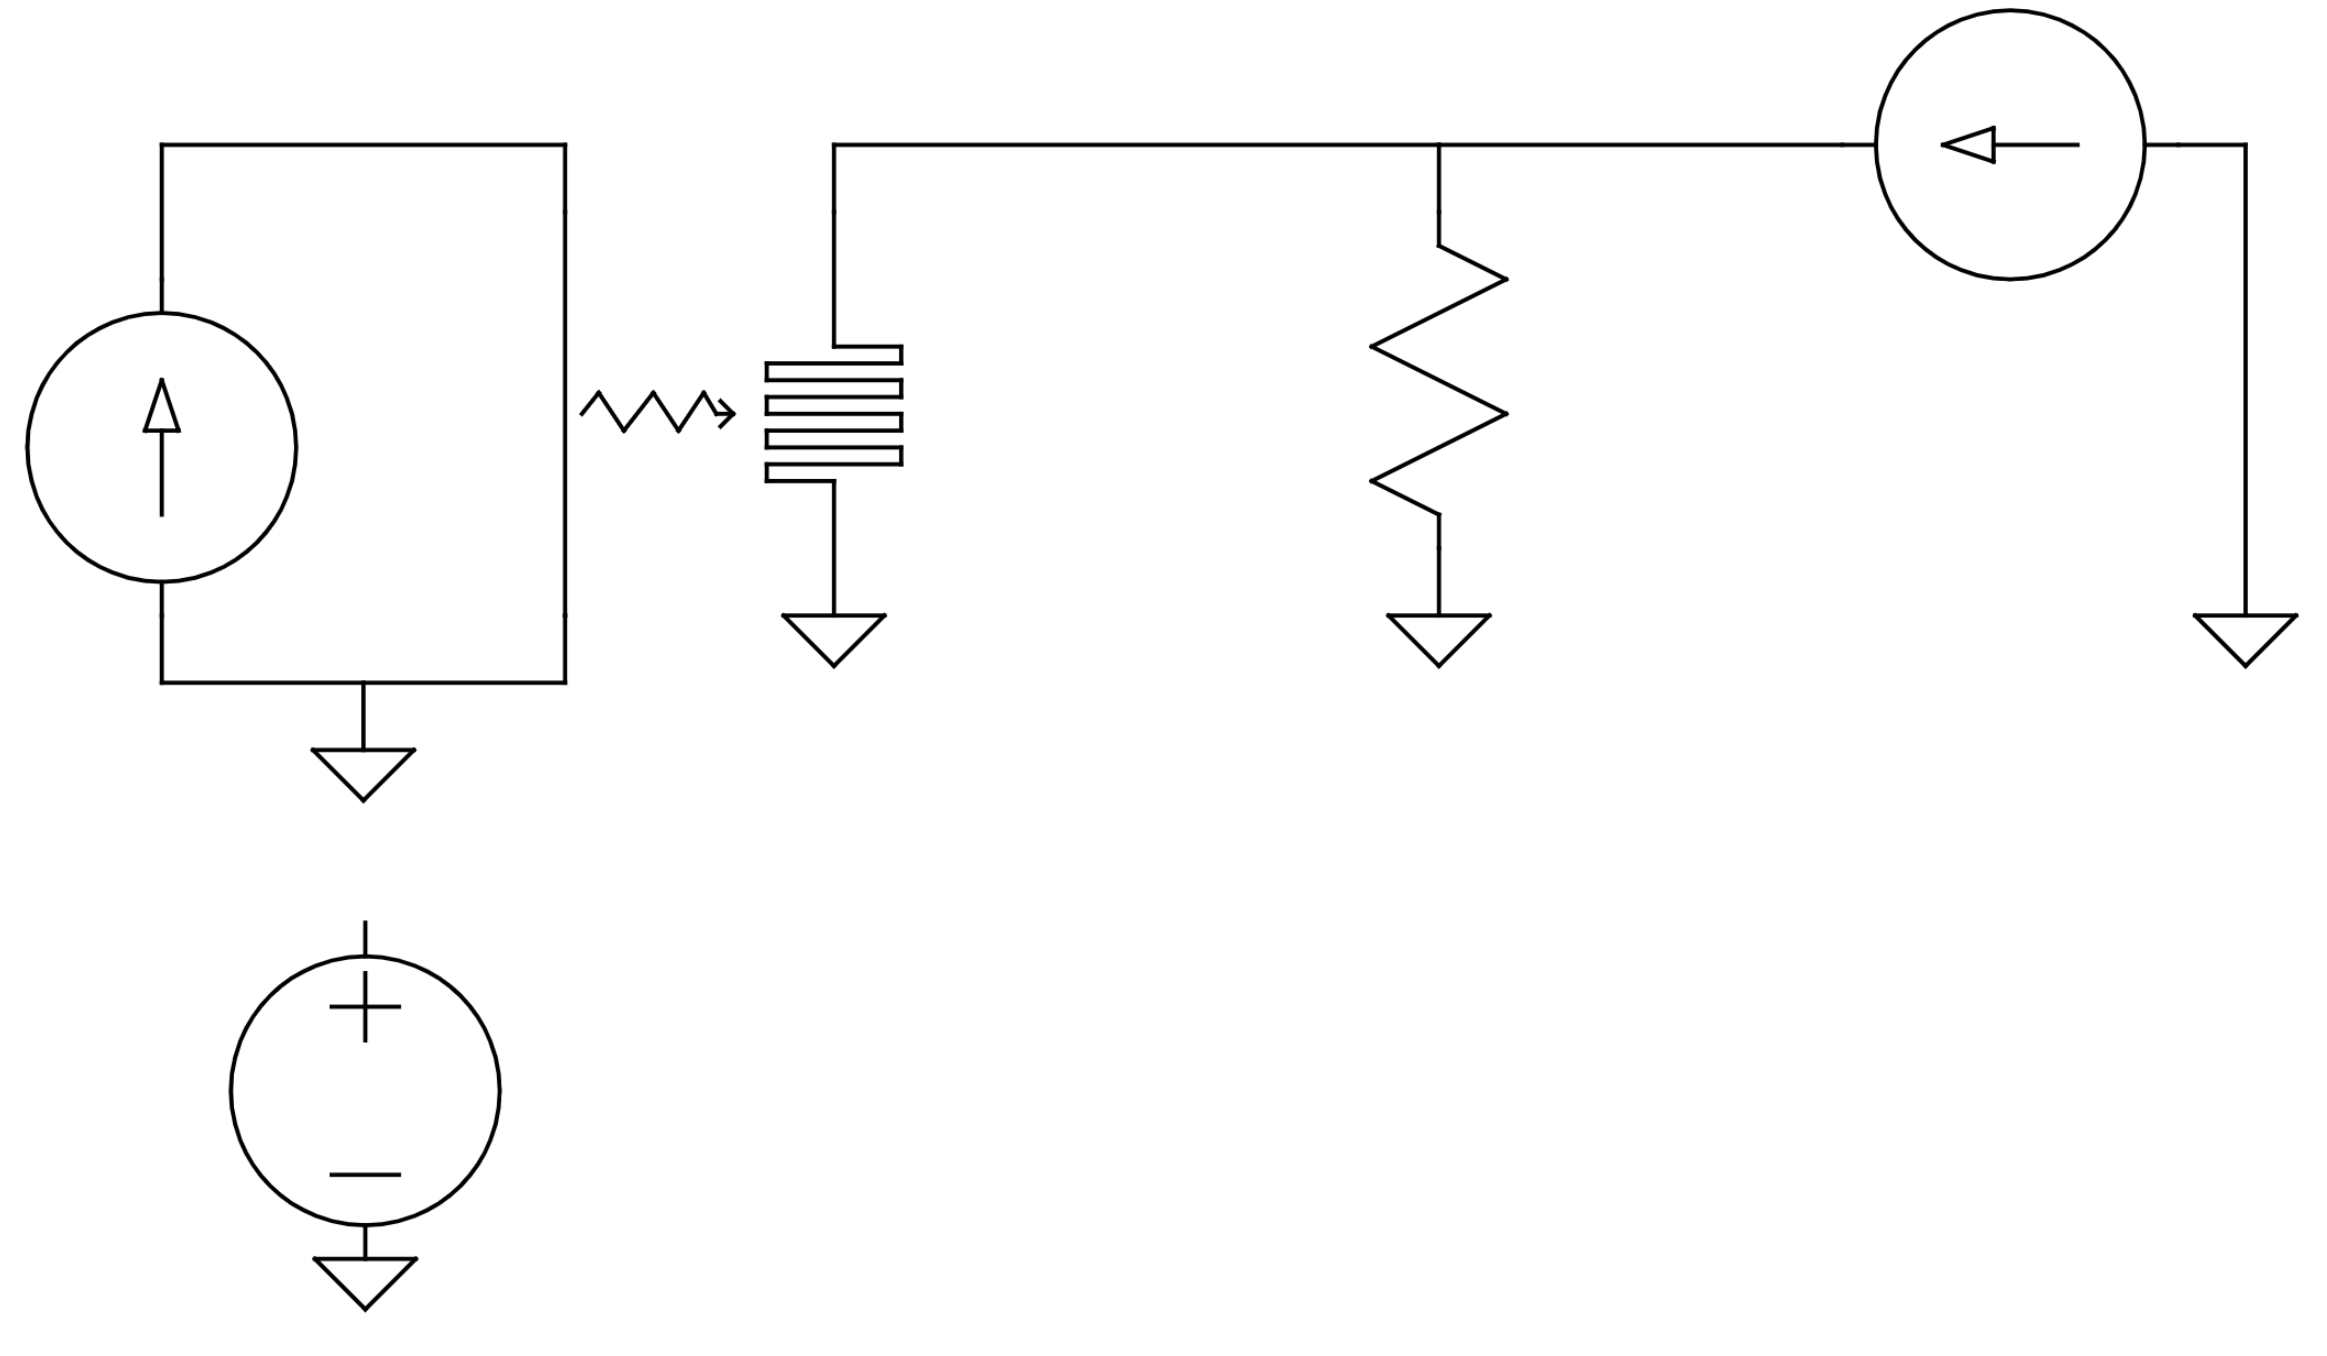
\includegraphics[width=0.4\textwidth]{figs/w_malicious_circ_diag.png}
    \label{fig:w_malicious_circ_diag}
    }
    \subfigure[]{
    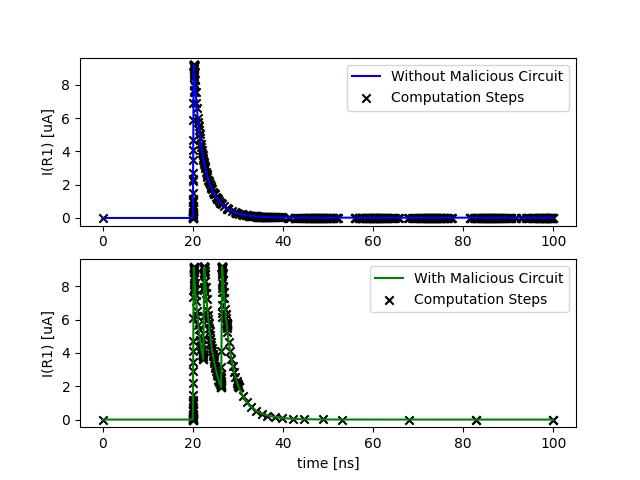
\includegraphics[width=0.55\textwidth]{figs/w_malicious_circ.png}
    \label{fig:w_malicious_circ}
    }
    \caption{(a) diagram of the circuit tested with a bias current of $11.1\mu$A and a photon incident at $20$ns on the existing nanowire model. The bottom circuit is a ``malicious circuit,'' it is a pulse source that produces a $10$ns square pulse during the evolution of the hotspot. (b) The top plot showcases a single hotspot forming when simulating
    the SNSPD circuit without the malicious circuit included. The bottom plot shows the evolution when the malicious circuit
    is included. The bottom plot shows multiple oscillations with peaks even though it should only show one. The
    malicious circuit projected errors on the hotspot evolution and caused the nanowire model to switch when it wasn't supposed to. The crosses indicate the individual timesteps the solver computed the waveform at.}
\end{figure}

Figure \ref{fig:w_malicious_circ_diag} shows a typical SNSPD readout circuit biased with $11.1\mu$A
and a decoupled
malicious voltage source. By running a simulation with and without that malicious subcircuit,
we get see how the inclusion of a malicious circuit can affect the output result in figure
\ref{fig:w_malicious_circ}. Note that the resulting solution is not possible given the
typical geometry, even though it looks plausible, since the period of oscillations is not 
regular. Since we know the malicious voltage source in no way affects the main circuit,
we know that our model is unstable over time steps taken by PULSE sources. Note that
not all bias currents misbehave, but by sweeping a range of bias values, we are able to
find a couple that don't work as shown in figure \ref{fig:sweepbias}. About $6\%$ of
bias values output inconsistent results for a sweep with between $11\mu$A and $12\mu$A 
in steps of $10$nA.

This method can be extended to detect the stability of linear systems by coupling
a non-linear discriminator $D$ to the circuit $C$ and testing the stability by simulating
$C+D+M$. The discriminator $D$ needs amplify $\varepsilon$ deviations, the most straight-forward
way of doing that projects a node value from $C$ onto a finite field. For instance $D$ 
could be a behavioural source with an expression similar to $V=\cf{IF}(\cf{n001}>10\mathrm{u}, 1, 0)$ 
to couple to node \cf{n001} in circuit $C$. $D$ should have no effect on the operation of $C$,
any operation change in $C$ is an indicator of instability of $C$.

\todooptional[]{fig: malicious circuit examples}

% \subsubsection{Proof of Equivalence to Stability}

\subsection{Improving the Nanowire Model}

\subsubsection{Current nanowire model}
\label{current_nw}

Berggren et al.'s nanowire model comprises of four sub-circuits outlined in figure \ref{fig:old_nw}. The main subcircuit (subcircuit a), consists of a
non-linear inductor in series with a b-source in parallel with a resistor.
The non-linear inductor simulates the continuously non-linearity due to kinetic inductance,
while the resistor and b-source simulate switching and hotspot dynamics.
Subcircuit (b) stores the value of the boolean state tracking 
whether the nanowire is in the normal or superconducting state.
Subcircuit (c) is the hotspot integrator, the subcircuit is the
circuit analog for the hotspot integral solving for the node voltage $v_3$
which represents the hotspot resistance. Subcircuit (d) is an input port for
photons.

\begin{figure}
    \centering
    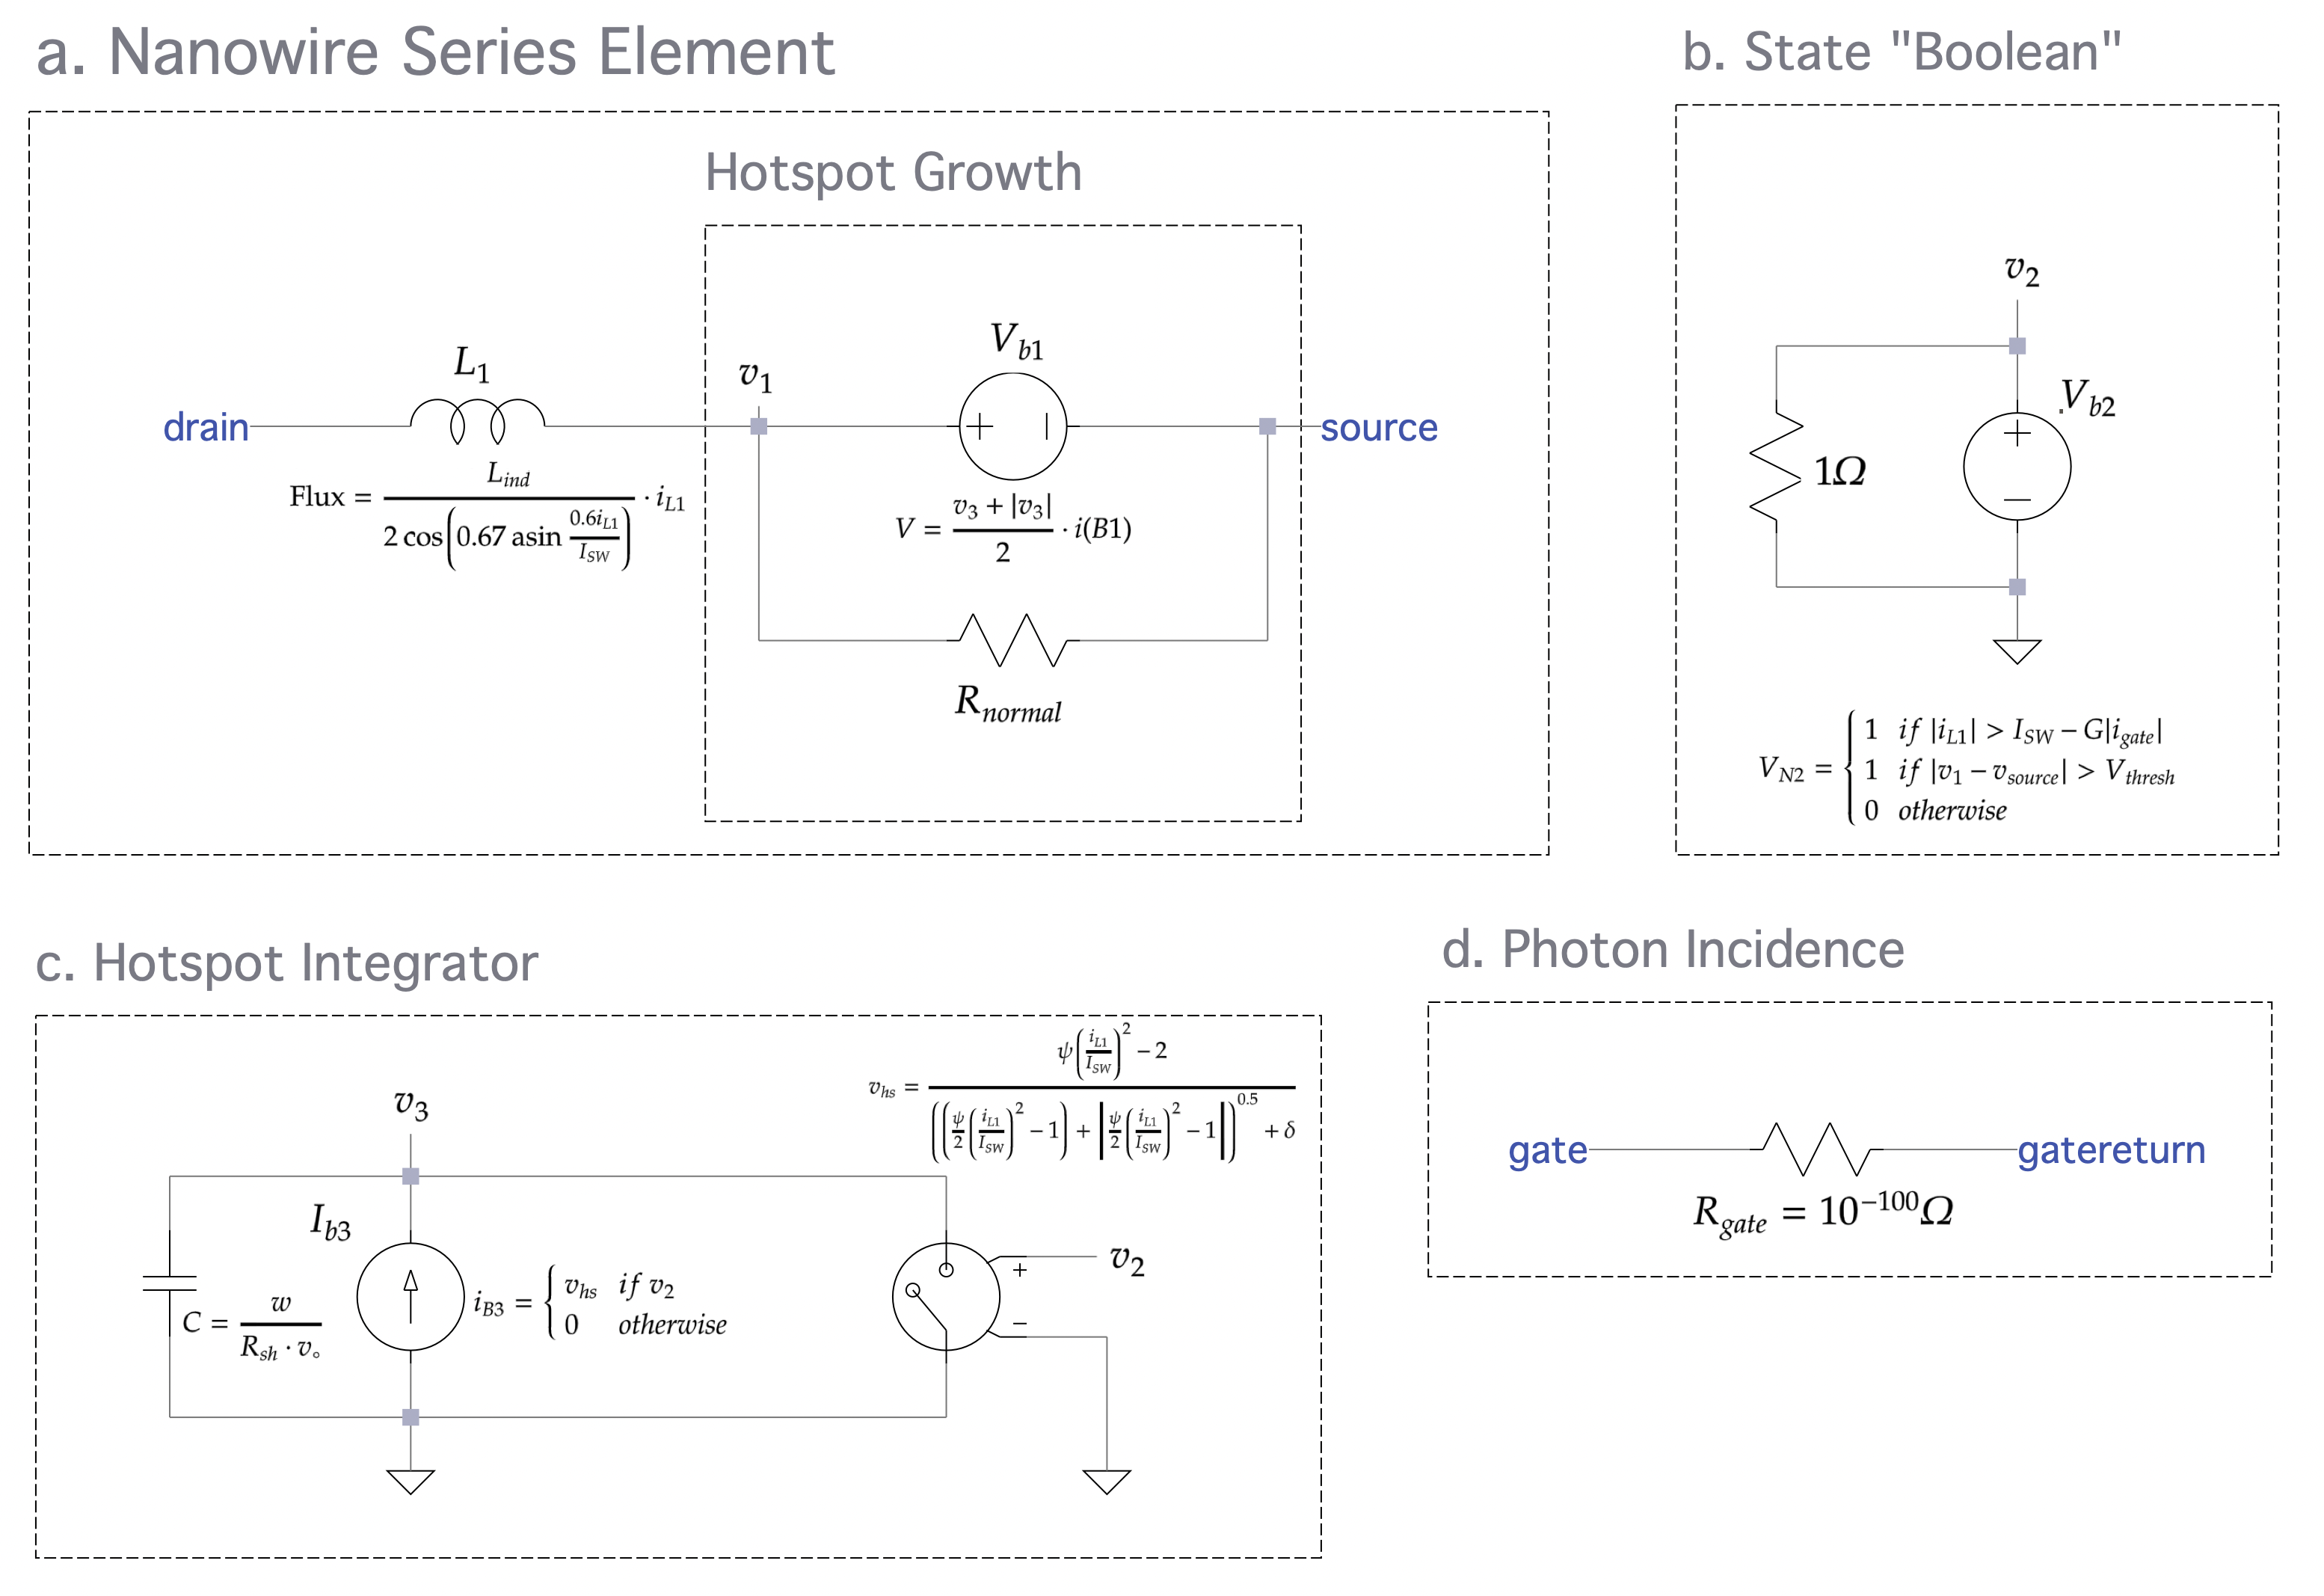
\includegraphics[width=\textwidth]{figs/old_nw.png}
    \caption{Diagram showcasing the four subcircuits used in the 
    Berggren et al. SPICE dynamic nanowire model. 
    Subcircuit a accounts for the kinetic inductance
    continuous non-linearity and the resistance in the normal state. Subcircuit b
    tracks a boolean state of superconducting vs. normal. Subcircuit c integrates
    the hotspot velocity as per the phenomenological hotspot model. Subcircuit
    d is the photon inlet.
    \todofig[inline]{remove the Rgate text from this fig}}
    \label{fig:old_nw}
\end{figure}

\begin{figure}
    \centering
    \begin{tikzpicture}[scale=1,auto=center,every node/.style={circle}]
      \tikzset{vertex/.style = {shape=circle,draw,minimum size=4em,fill=white}}
        \tikzset{edge/.style = {->,> = latex'}}
        \def\size{8em}
        % vertices
        \node[vertex] (b1) at  (360/7 * 0:\size) {$V_{b1}$};
        \node[vertex] (n1) at  (360/7 * 1:\size) {$v_1$};
        \node[vertex] (n2) at  (360/7 * 2:\size) {$v_2$};
        \node[vertex] (n3) at  (360/7 * 3:\size) {$v_3$};
        \node[vertex] (r3) at (360/7 * 4:\size) {$i_{gate}$};
        \node[vertex] (s1) at (360/7 * 5:\size) {\small{switch}};
        \node[vertex] (l1) at (360/7 * 6:\size) {$L_1$};
        %edges
        \draw[edge] [loop right] (b1) to (b1);
        \draw[edge] (b1) to (n1);
        \draw[edge] (n1) to (n2);
        \draw[edge] (n2) to (n3);
        \draw[edge] (n2) to (s1);
        \draw[edge] (n3) to (b1);
        \draw[edge] (r3) to (n2);
        \draw[edge] (s1) to (n3);
        \draw[edge] (l1) to (n2);
        \draw[edge]  (l1) to (n3);
    \end{tikzpicture}
    \caption{A dependency graph for some elements and nodes of the nanowire model as presented in
    figure \ref{fig:old_nw}. Each node in the graph represents
    a circuit node value that is calculated or an element parameter.
    Since the compiler is a black box,
    some degree and outdegree $1$ nodes were removed. Note that the time dependence
    of parameters is also removed, i.e. an edge to a variable could represent
    dependence in the same timestep or on the previous timestep of the value.
    This is a heuristic of how simulation parameters
    are dependent on each other, i.e. how stiffness or errors in one graph node couple to other nodes.}
    \label{fig:dependency_graph}
\end{figure}

Using dependency graphs, we can visualize how the model elements
are correlated in figure \ref{fig:dependency_graph}. 
By using directed graphs to represent execution 
order for nodes and element values, we can visualize the dependece
of parameters on each other. A system is said to have a dependency graph $G = (V, E)$
where $V$ represents variables as nodes and $E$ are the dependency edges.
A set of variables $V_1, V_2 \subseteq V$ are said to be decoupled if all nodes
in $V_1$ have node edges pointing to $V_2$ and vice versa. The dependency
graph for a system highlights how projection errors integrate over time.
\todoexplain[]{Explain why cycle, why thermal integrator projections...}
\todoref[]{citation from book Software Testing and Analysis: Process, Principles, and Techniques. Chapter 6}
\todoref[]{dragon book??}
%http://www.cs.toronto.edu/~chechik/courses16/csc410/dataflowReadings.pdf

The current nanowire model also currently lacks a DC part (operational mode) 
of the model.
LTspice DC solver struggles to efficiently represent a nanowire thats
undergoing relaxation oscillations (the solver tends to find that it is
switched) and misrepresents DC solutions for the superconducting state
as the normal state. This implies that for nanowire simulations,
the initial state of everything must be zero since transient analysis relies
on operational point analysis beforehand. Namely, all bias sources,
DC or not, should start at $0$. So a DC bias would be a \cf{PULSE} starting
at 0, ramping to a value and let it rest there for a bit. This is a by-product 
of LTspice not recognizing meta-stable systems. This is tackled by the new 
simulator introduced in section \ref{julia-sim-chapter}.

\subsubsection{Stability of the original nanowire model}

By varying the relative tolerance and testing different geometries, the value $10^{-6}$
seems to perform the best in terms of stability and accuracy. By testing the LC tank
geometry shown in \ref{fig:tank_circ} using a nanowire and swapping it with a linear 
inductor, we can test several \cf{reltol} values and see if we see the expected 
oscillation behaviour. Intuitively, as the relative tolerance value used gets smaller,
the circuit should be ``more correct'' than when allowing for a bigger tolerance.
For the nanowire model, we don't see that behaviour. Relative tolerances between $10^{-3}$
and $10^{-7}$
consistently worked in our tests, producing a sinusoidal oscillation. Values
above $10^{-7}$ either switch into the resistive state and lose all the energy immideatly
or oscillate in a decaying fashion. Meanwhile, for the SNSPD readout configuration,
we see consistently better behaviour using the malicious circuits method presented in
\ref{malicious_circuits} as we go from $10^{-3}$ to $10^{-6}$ across photon events
and relaxation oscillations.

Even with a \cf{reltol} value of $10^{-6}$, the existing nanowire model is highly unstable
and can be improved through stability analysis.
Using Malicious Circuits, we test multiple operation regimes for
the nanowire and study the stability of every sub-circuit separately. Namely,
we care about the nanowire behavior in 4 different regimes: 
(1) as an inductor and resistor when normal, 
(2) as an inductor when superconducting, (3) the hotspot evolution when a photon is
incident, and (4) relaxation oscillation regime. We test these different regimes 
using one circuit with one nanowire element across \cf{reltol} values of $10^{-3}$
and $10^{-6}$ and compare it to the expected solution.

\subsubsection{Different Integrator}

The malicious circuits analysis on the old model indicated
that the integrator circuit is the main source of instability. 
We replaced it with a behavioral source that integrates the same hotspot
and observed an improvement in overall behavior.
This model is mathematically identical to the previous one with 2 changes
to the implementation: (1) use a built-in integrator instead of the circuit
integrator (subcircuit c) and (2) replacing $\frac{x+|x|}{2}$ with a conditional
on $x>0$ (or bound $x$ by the \cf{limit}).

The LTspice built-in integrator is better handled
by spice than the integrator's circuit equivalent model.
It involves doing one operation instead of increasing the circuit
matrix size. 
This not only involves creating fewer projections onto the circuit (leading to less errors)
but using the built-in integrator allows LTspice to better keep track of integration
time and shorting to ground. Note that the new integrator using the built-in
\cf{sdt} math command uses a reset condition. This condition is better handles as it
doesn't involve decreasing the timestep in a projective fashion as with circuit
non-linearities. The reset condition is substituting the switch that shorts $v_3$
to ground in figure \ref{fig:old_nw}. When the $v_2=0$ (wire is superconducting),
the integrator resets to the initial condition $0$.

The previous nanowire model also involved the switch toggling between the off and on
state with resistances of $1$m$\Omega$ and $10$G$\Omega$. This switching behaviour
introduces a strong non-linearity that can be better handled by the reset method
used by the \cf{sdt} command. In SPICE, a resistance changing value by an order of
$10^6$ instantly is unstable, let alone a magnitude of $10^{15}$. This magnitude
change coupled with using a lower \cf{reltol} leads to a large instability that
should be avoided.

\begin{figure}
    \centering
    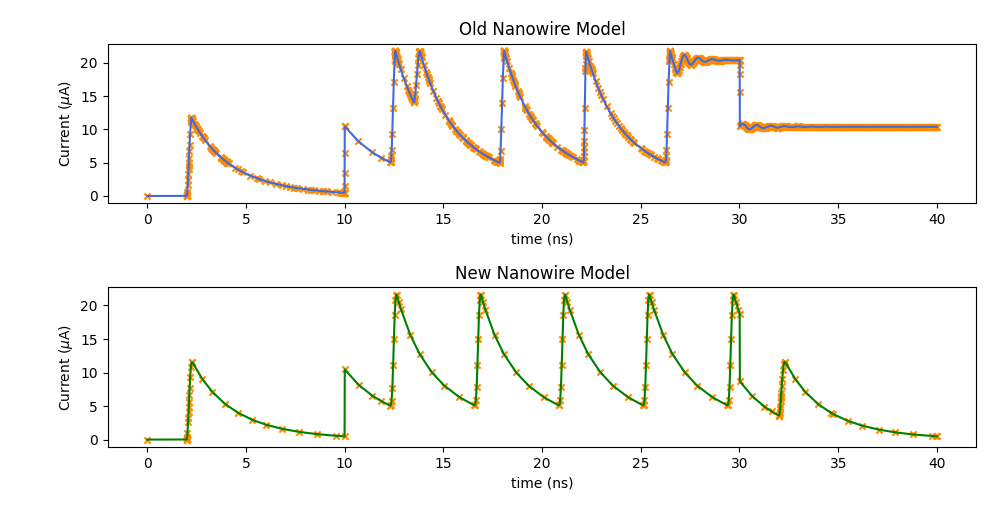
\includegraphics[width=0.9\textwidth]{figs/int_improvement_1e-3.png}
    \caption{Comparison of the old and new nanowire model that replaces the
    circuit integrator with the internal LTspice resetting integrator. Solid
    lines represent the output waveform and the crosses are the values evaluated at each
    individual timestep. Photons are incident at $2$ and $32$ns on a wire biased by $15\mu$A.
    The bias is increased to $25\mu$A between $10$ and $30$ns to enter the wire into the
    relaxation oscillation regime.We see that in this example, the new model is more accurate, as well as,requiring less discrete timesteps to solve the equation at.}
    \label{fig:int_improvement_1e-3}
\end{figure}

\begin{figure}
    \centering
    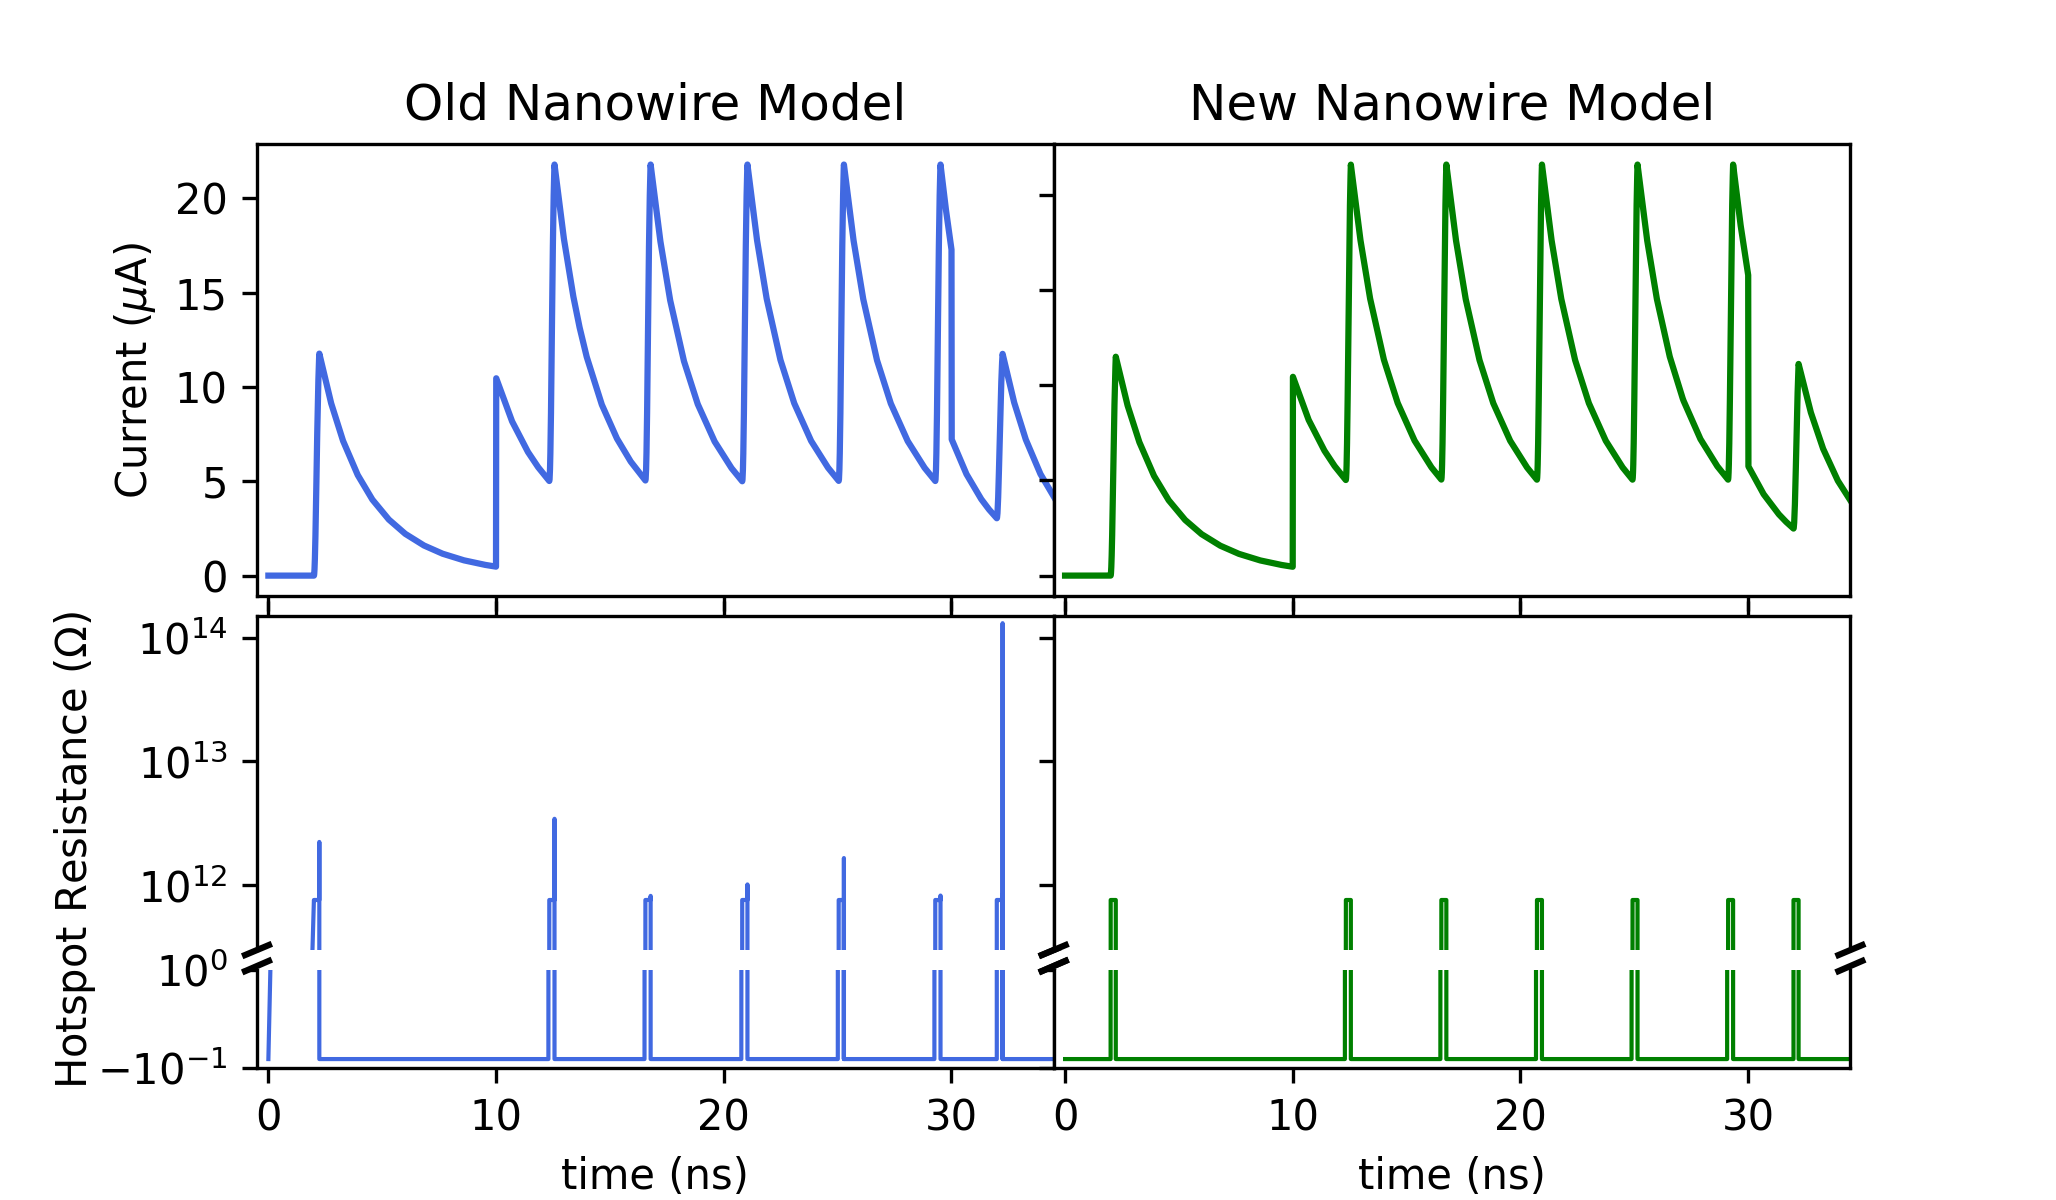
\includegraphics[width=0.9\textwidth]{figs/int_improvement_1e-6.png}
    \caption{For the same setup in figure \ref{fig:int_improvement_1e-3}, we see
    that both models seem to perform well on readout when using a \cf{reltol} value
    of $10^{-6}$. However, the hotspot resistance is unstable in the old model peaking
    up to $2$ orders of magnitude above the actual value.}
    \label{fig:int_improvement_1e-6}
\end{figure}

Along with more accurate simulations of the behavior of the nanowire, we also
observe the simulator using fewer time steps overall (fewer crosses in figure 
\ref{fig:int_improvement_1e-3}). This corresponds to faster convergence and also is
an indicator of fewer projections that needed to be done, indicating less
error over the binary state. Needing fewer points to solve a system suggests
linearity. In this case, we can observe that the model can comfortably relax
back into linearity when the pulse magnitude is constant and there is no
switching behavior occurring, however, when switching, more data points are used up.

Figure \ref{fig:int_improvement_1e-6} compares the performance of the old and new 
nanowire models at a \cf{reltol$=10^{-6}$}. This example is for the same bias as in 
figure \ref{fig:int_improvement_1e-3}, where the current output seems correct.
However, looking at the hotspot resistance by scoping the internal variables of the 
model, we see that the hotspot resistance has huge spikes, up to 2 orders of magnitude
above the correct value. This is a source of instability in the model that can also
be analyzed using Malicious Circuits, even though the hotspot resistance itself is
a combined measurable ($R_{\mathrm{hotspot}} = \frac{v_1 - v_{\mathrm{source}}}{i}$).

\begin{figure}
    \centering
    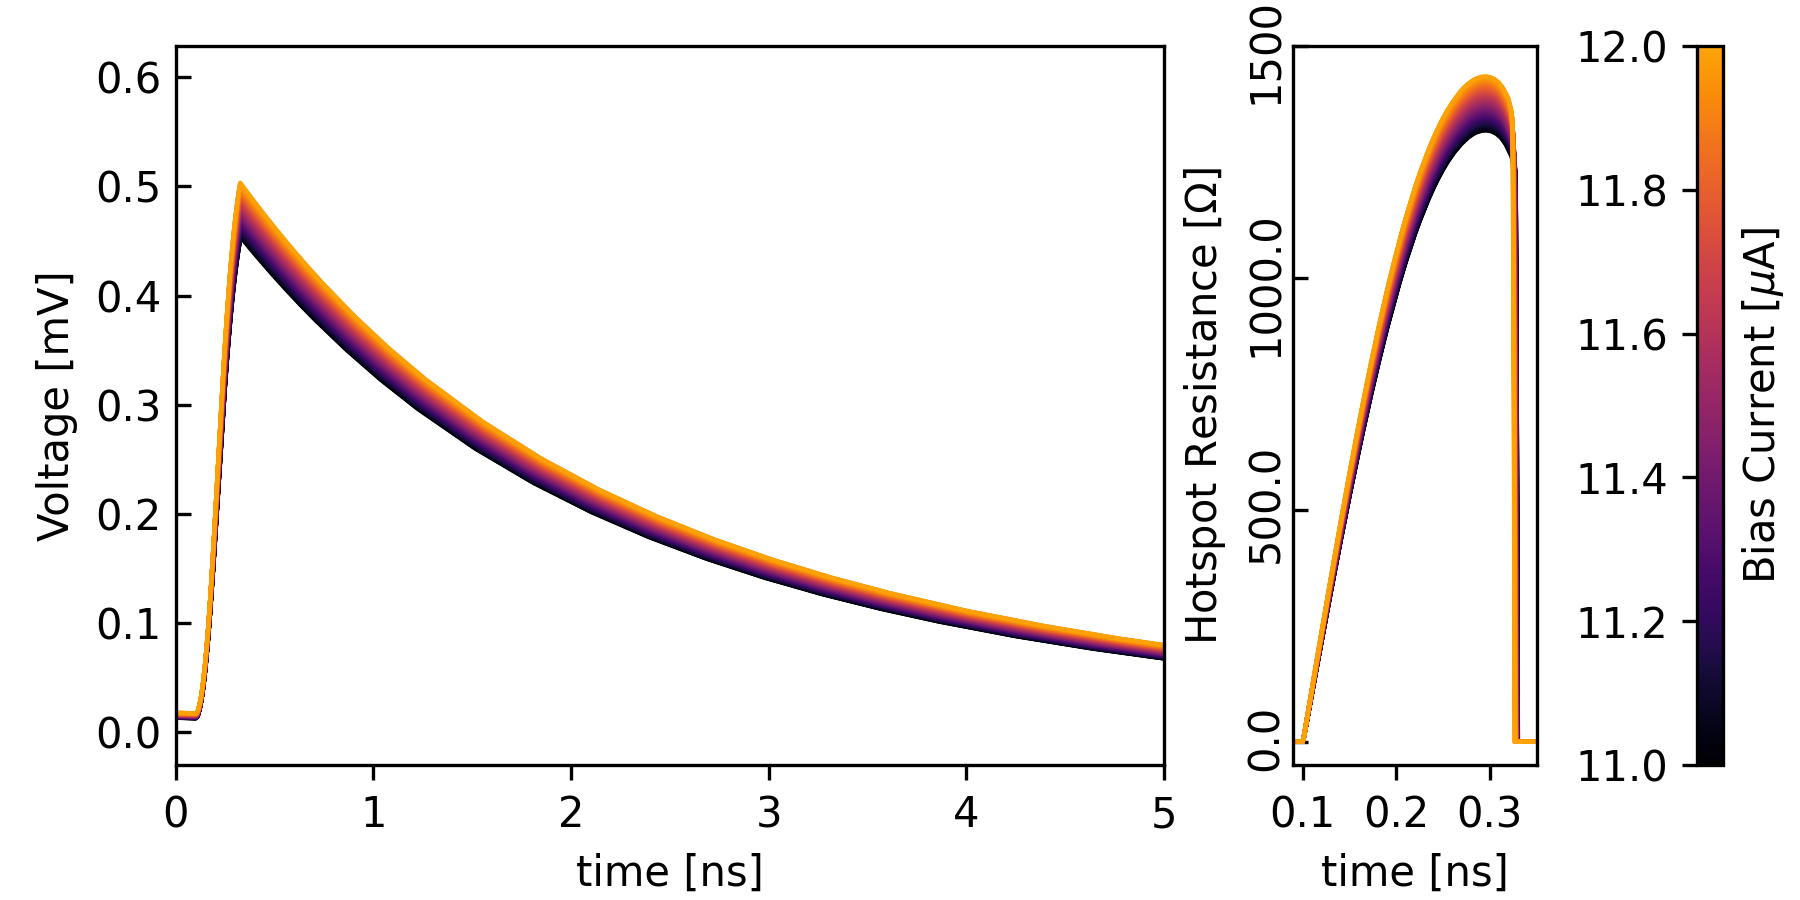
\includegraphics[width=0.8\textwidth]{figs/not_jumbled_mess.png}
    \caption{A sweep of bias currents on the new nanowire model with a photon detection event.
    $100$ equally spaced bias values between $11\mu$A and $12\mu$A were tested. We observe
    a smooth gradient of the resultant
    hotspot resistance and voltage spike that is much more consistent than the old nanowire
    as shown in figure \ref{fig:sweepbias}. 
    }
    \label{fig:not_jumbled_mess}
\end{figure}

[TODO] Compare figure \ref{fig:not_jumbled_mess} to the original figure \ref{fig:sweepbias}.
Notice how a higher resistance max value corresponds to a faster decay - probably the current
being routed into the inductor faster.

Talk about choosing between bounding with limit and if(x) instead of $x+|x|$

\subsubsection{1 Element Models}

\subsubsection{0 Resistance Models}